\section{Le Froid}

\begin{frame}{Le Froid — Causes et Mécanismes}
    \begin{columns}
        \begin{column}{0.55\textwidth}
            \textbf{Pourquoi a-t-on froid ?}
            \begin{itemize}
                \item L'eau conduit la chaleur \textbf{25 fois plus vite} que l'air.
                \item \textbf{La Température d'Équilibre :}
                \begin{itemize}
                    \item Dans l'eau, la neutralité thermique est à \textbf{33$^\circ$C}.
                    \item En dessous de 33$^\circ$C, le corps perd inévitablement de la chaleur s'il n'est pas protégé.
                \end{itemize}
                \item Température corporelle ($\approx 37^\circ C$) $>$ Température de l'eau.
            \end{itemize}
            
            \textbf{Le rôle de l'eau (voir schéma) :}
            \begin{itemize}
                \item L'eau circule dans la combinaison et "emporte" les calories.
                \item Le corps transmet sa chaleur à l'eau ambiante.
            \end{itemize}
        \end{column}
        
        \begin{column}{0.45\textwidth}
            \begin{figure}
                \centering
                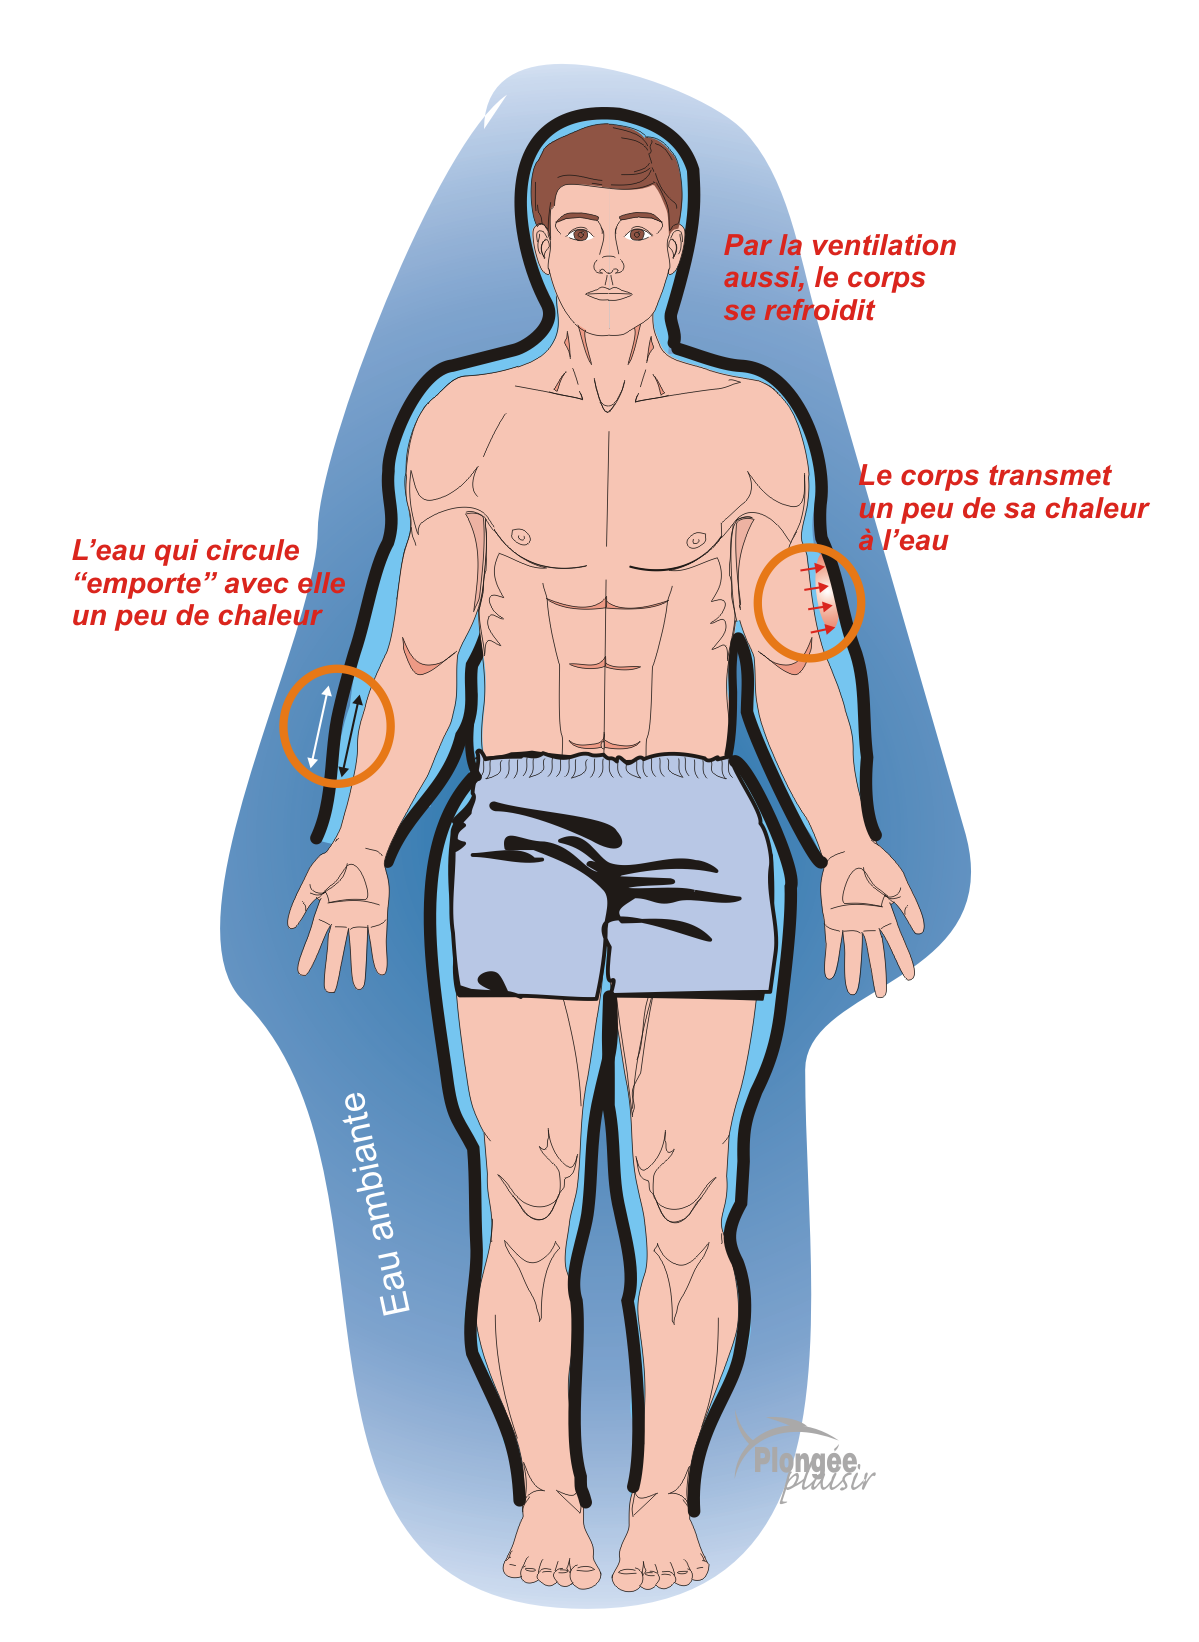
\includegraphics[height=0.85\textheight]{images/froid_circulation_eau}
            \end{figure}
        \end{column}
    \end{columns}
\end{frame}

\begin{frame}{Le Froid — Réactions physiologiques et Symptômes}
    \textbf{Mécanismes de défense (Signes d'alerte) :}
    \begin{itemize}
        \item \textbf{Frissons et claquements de dents :} Travail musculaire involontaire pour produire de la chaleur.
    \end{itemize}

    \vspace{-0.2cm} % Remonte légèrement les colonnes

    \begin{columns}[T] % T = alignement en haut
        \begin{column}{0.58\textwidth}
            \begin{itemize}
                \item \textbf{Diurèse d'immersion :} Envie pressante d'uriner (réaction au froid et à la pression).
                \item \textbf{Ventilation accélérée :} Conséquence de l'effort thermique.
            \end{itemize}

            \vspace{0.4cm}

            \textbf{Signes de gravité (Hypothermie marquée) :}
            \begin{itemize}
                \item Engourdissement des extrémités.
                \item Baisse de la tension artérielle.
                \item Risque d'arythmie, syncope, voire arrêt cardiaque.
            \end{itemize}
        \end{column}

        \begin{column}{0.40\textwidth}
            \centering
            % keepaspectratio évite de déformer l'image
            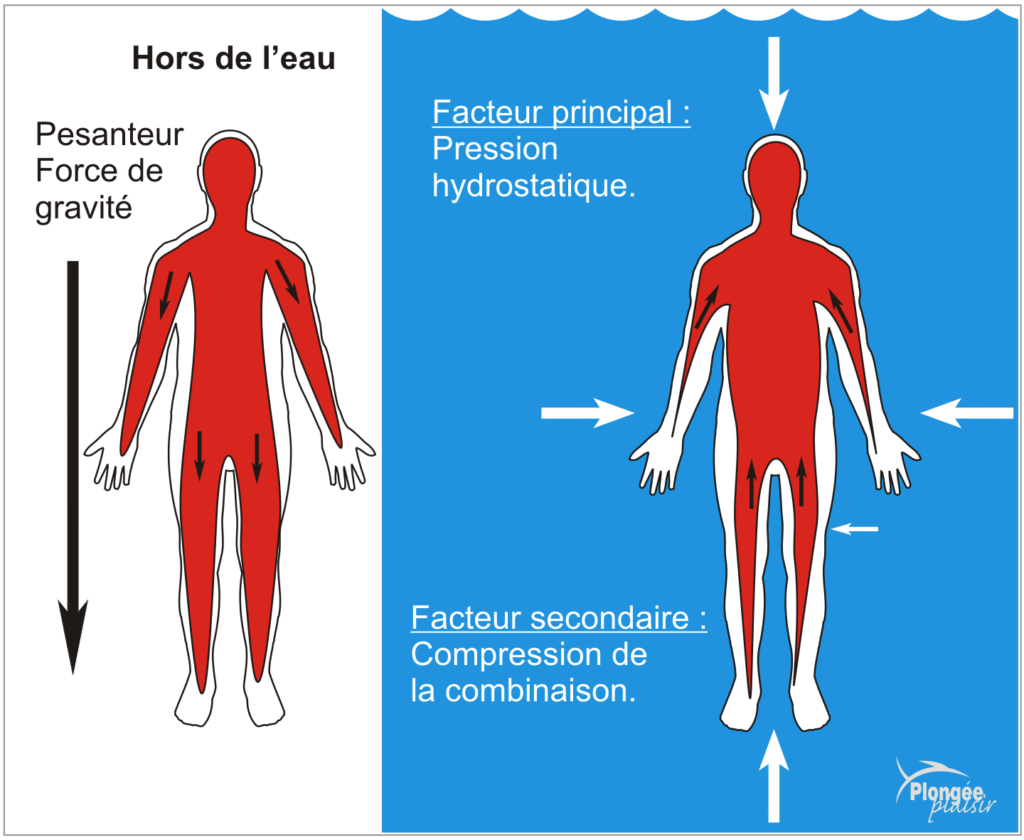
\includegraphics[height=0.6\textheight, keepaspectratio]{images/diurese_deshydratation}
        \end{column}
    \end{columns}
\end{frame}

\begin{frame}{Le Froid — Conséquences et Risques Connexes}
    Le froid n'est pas seulement inconfortable, il favorise d'autres accidents :
    
    \begin{alertblock}{Facteur favorisant de :}
        \begin{itemize}
            \item \textbf{L'Essoufflement :} Car le froid accélère le rythme ventilatoire.
            \item \textbf{L'ADD (Accident de Désaturation) :} 
                \begin{itemize}
                    \item Mauvaise élimination de l'azote due à la vasoconstriction (mauvaise circulation périphérique).
                    \item Saturation accrue si essoufflement.
                \end{itemize}
            \item \textbf{La Noyade :}
                \begin{itemize}
                    \item Perte du détendeur suite aux claquements de dents.
                    \item Difficulté à gérer son matériel à cause de l'engourdissement des mains.
                \end{itemize}
        \end{itemize}
    \end{alertblock}
\end{frame}

\begin{frame}{Prévention et Conduite à Tenir (CAT)}
    \begin{columns}[t] % Aligné en haut
        
        \begin{column}{0.48\textwidth}
            \textbf{\textcolor{blue}{PRÉVENTION (Avant/Pendant)}}
            \begin{itemize}
                \item \textbf{Équipement :}
                    \begin{itemize}
                        \item Combinaison ajustée (limiter la circulation d'eau).
                        \item \textbf{Cagoule :} Indispensable (30\% de perte par la tête).
                    \end{itemize}
                \item \textbf{Organisation :}
                    \begin{itemize}
                        \item Manger énergétique avant.
                        \item Surveillance mutuelle de l'équipement.
                        \item Accord : "J'ai froid" = Fin de plongée.
                    \end{itemize}
            \end{itemize}
        \end{column}

        \begin{column}{0.48\textwidth}
            \textbf{\textcolor{red}{RÉACTION (Si froid avéré)}}
            \begin{itemize}
                \item \textbf{Sous l'eau :}
                    \begin{itemize}
                        \item Apparition de frissons = \textbf{Fin de plongée}.
                    \end{itemize}
                \item \textbf{En surface :}
                    \begin{itemize}
                        \item Sécher et couvrir (Bonnet, couverture de survie).
                        \item Protéger du vent (Coupe-vent).
                        \item Boisson chaude et sucrée.
                    \end{itemize}
            \end{itemize}
        \end{column}
        
    \end{columns}

    \vspace{0.4cm}

    \begin{alertblock}{À NE PAS FAIRE}
        \centering
        \textbf{NE PAS FRICTIONNER} (risque de retour veineux froid) \\
        \textbf{JAMAIS D'ALCOOL} (aggrave l'hypothermie)
    \end{alertblock}
\end{frame}